\documentclass[10pt]{extarticle}
\title{Analysis 2 Notes}
\author{Giacomo Ellero}
\date{Semester 2, 2023/2024}

\usepackage{amsfonts}
\usepackage{amsthm}
\usepackage{amssymb}
\usepackage{amsmath}
\usepackage{mathtools}
\usepackage{commath}
\usepackage{dirtytalk}
\usepackage{parskip}
\usepackage{mathrsfs}
\usepackage[many]{tcolorbox}
\usepackage{xparse}
\usepackage[a4paper,margin=1.5cm]{geometry}
\usepackage{bookmark}
\usepackage{physics}
\usepackage{tikz}
\usepackage{capt-of}
\usepackage{subfig}
\usepackage{cancel}
\usepackage{float}

\newcommand{\C}{\mathbb{C}}
\newcommand{\R}{\mathbb{R}}
\newcommand{\N}{\mathbb{N}}
\newcommand{\F}{\mathcal{F}}
\renewcommand{\Re}{\operatorname{Re}}
\renewcommand{\Im}{\operatorname{Im}}
\newcommand{\munderbar}[1]{\underbar{\ensuremath{#1}}}
\newcommand{\skiplineafterproof}{$ $\par\nobreak\ignorespaces}


\newenvironment{absolutelynopagebreak}
  {\par\nobreak\vfil\penalty0\vfilneg
   \vtop\bgroup}
  {\par\xdef\tpd{\the\prevdepth}\egroup
   \prevdepth=\tpd}

\newtcolorbox{examplebox}[1]{colback=green!5!white,colframe=green!40!black,title={#1},fonttitle=\bfseries,parbox=false}
\newtcolorbox{notebox}[1]{colback=blue!5!white,colframe=blue!40!black,title={Note: #1},fonttitle=\bfseries,parbox=false}
\newtcolorbox{bluebox}[1]{colback=blue!5!white,colframe=blue!40!black,title={#1},fonttitle=\bfseries,parbox=false}
\newtcolorbox{warningbox}[1]{colback=orange!5!white,colframe=orange!90!black,title={Warning: #1},fonttitle=\bfseries,parbox=false}
   
\begin{document}

\maketitle
\tableofcontents
\clearpage

\section{Class of 12/02/2024}

In this class we will discuss mainly multi-variable calculus:
\begin{itemize}
    \item Parametric curves: $\R \to \R^d$.
    \item Graphs: $\R^2 \to \R$.
    \item Vector fields: $\R^d \to \R^d$.
\end{itemize}

And in general we will discuss functions $f: \R^d \to \R^p$.

$\R^d$ is a vector space, like the ones we have seen in linear algebra, so many notions carry over.

\subsection{Dot product and distance}

\textbf{\underline{Definition} (dot product)}: Let $\munderbar{x}, \munderbar{y} \in \R^d$. The dot product of $x$ and $y$ is defined as

$$
    \munderbar{x} \cdot \munderbar{y} = \sum_{i=1}^d x_i y_i
$$

We have seen dot products (inner products) in linear algebra but we will see some of their proprieties again:
\begin{enumerate}
    \item $\munderbar{x} \cdot \munderbar{y} = \munderbar{y} \cdot \munderbar{x}$.
    \item $\munderbar{x} \cdot (\munderbar{y} + \munderbar{z}) = \munderbar{x} \cdot \munderbar{y} + \munderbar{x} \cdot \munderbar{z}$.
    \item $\munderbar{x} \cdot \munderbar{x} \geq 0$ and $\munderbar{x} \cdot \munderbar{x} = 0 \iff \munderbar{x} = \munderbar{0}$.
\end{enumerate}

\subsubsection{Norm}

\textbf{\underline{Definition} (norm)}: Let $\munderbar{x} \in \R^d$. The norm of $\munderbar{x}$ is defined as

$$
    \norm{\munderbar{x}} = \sqrt{\munderbar{x} \cdot \munderbar{x}}
$$

For a more general definition see the linear algebra notes.

\subsection{Cauchy-Schwarz inequality}

\textbf{\underline{Theorem} (Cauchy-Schwarz inequality)}: Let $\munderbar{x}, \munderbar{y} \in \R^d$. Then

$$
    \abs{\munderbar{x} \cdot \munderbar{y}} \leq \norm{\munderbar{x}} \norm{\munderbar{y}}
$$

\begin{proof}
    We introduce $f(t) = \norm{\munderbar{x} + t \munderbar{y}}^2$.

    We apply some algebraic manipulation to $f(t)$ according to the proprieties of the dot product and the norm:

    \begin{align*}
        f(t) & = \norm{\munderbar{x} + t \munderbar{y}}^2                                                                                                              \\
             & = (\munderbar{x} + t \munderbar{y}) \cdot (\munderbar{x} + t \munderbar{y})                                                                             \\
             & = \munderbar{x} \cdot (\munderbar{x} + t \munderbar{y}) + t \munderbar{y} \cdot (\munderbar{x} + t \munderbar{y})                                       \\
             & = \munderbar{x} \cdot \munderbar{x} + t \munderbar{x} \cdot \munderbar{y} + t \munderbar{y} \cdot \munderbar{x} + t^2 \munderbar{y} \cdot \munderbar{y} \\
             & = \norm{\munderbar{x}}^2 + 2t \munderbar{x} \cdot \munderbar{y} + t^2 \norm{\munderbar{y}}^2
    \end{align*}

    If $\munderbar{y} \ne 0$ we have that $f(t)$ is a parabola which is always positive, hence $\Delta \leq 0$. We have

    \begin{align*}
        \Delta & = (2 \munderbar{x} \cdot \munderbar{y})^2 - 4 \norm{\munderbar{x}}^2 \norm{\munderbar{y}}^2        \\
               & = 4 (\munderbar{x} \cdot \munderbar{y})^2 - 4 \norm{\munderbar{x}}^2 \norm{\munderbar{y}}^2 \leq 0 \\
    \end{align*}

    We pass to the inequality and we get

    \begin{align*}
        \cancel{4}(\munderbar{x} \cdot \munderbar{y})^2 & \leq \cancel{4} \norm{\munderbar{x}}^2 \norm{\munderbar{y}}^2 \\
        \abs{\munderbar{x} \cdot \munderbar{y}} ^2      & \leq \norm{\munderbar{x}}^2 \norm{\munderbar{y}}^2            \\
        \abs{\munderbar{x} \cdot \munderbar{y}}         & \leq \norm{\munderbar{x}} \norm{\munderbar{y}}
    \end{align*}
\end{proof}

Note that if $\Delta = 0$ it's easy to prove that $\munderbar{x}$  = t $\munderbar{y}$, hence they are linearly dependent. This is the only case in which the inequality becomes an equality.

\subsection{Defining the angle between two vectors}

\textbf{\underline{Definition} (angle)}: Let $\munderbar{x}, \munderbar{y} \in \R^d$. The following relation holds between the dot product and the angle $\theta$ between the two vectors:

$$
    \munderbar{x} \cdot \munderbar{y} = \norm{\munderbar{x}} \norm{\munderbar{y}} \cos \theta
$$

hence

$$
    \theta = \arccos \left( \frac{\munderbar{x} \cdot \munderbar{y}}{\norm{\munderbar{x}} \norm{\munderbar{y}}} \right)
$$

From the definition we get that $\munderbar{x} \cdot \munderbar{y} = 0 \iff \theta = \frac{\pi}{2}$.

Cauchy-Schwarz inequality guarantees that the argument of $\arccos$ is always between -1 and 1.

Note that this is a definition, not a theorem: we are defining the concept of angle from the dot product.

\section{Class of 14/02/2024}

These theorems have been covered already in linear algebra, see the notes for more details.

\subsection{Triangle inequality}

\textbf{\underline{Theorem} (triangle inequality)}: Let $\munderbar{x}, \munderbar{y} \in \R^d$. Then

$$
    \norm{\munderbar{x} + \munderbar{y}} \leq \norm{\munderbar{x}} + \norm{\munderbar{y}}
$$

\begin{proof}
    We have that

    \begin{align*}
        \norm{\munderbar{x} + \munderbar{y}}^2 & = (\munderbar{x} + \munderbar{y}) \cdot (\munderbar{x} + \munderbar{y})                                                                         \\
                                               & = \munderbar{x} \cdot (\munderbar{x} + \munderbar{y}) + \munderbar{y} \cdot (\munderbar{x} + \munderbar{y})                                     \\
                                               & = \munderbar{x} \cdot \munderbar{x} + \munderbar{x} \cdot \munderbar{y} + \munderbar{y} \cdot \munderbar{x} + \munderbar{y} \cdot \munderbar{y} \\
                                               & = \norm{\munderbar{x}}^2 + 2 \munderbar{x} \cdot \munderbar{y} + \norm{\munderbar{y}}^2
    \end{align*}

    We apply the Cauchy-Schwarz inequality and we get

    \begin{align*}
        \norm{\munderbar{x} + \munderbar{y}}^2 & \leq \norm{\munderbar{x}}^2 + 2 \norm{\munderbar{x}} \norm{\munderbar{y}} + \norm{\munderbar{y}}^2 \\
        \norm{\munderbar{x} + \munderbar{y}}^2 & \leq \left(\norm{\munderbar{x}} + \norm{\munderbar{y}}\right)^2
    \end{align*}

    We take the square root of both sides and we get the result.
\end{proof}

\subsection{Pythagorean theorem}

\textbf{\underline{Theorem} (Pythagorean theorem)}: Let $\munderbar{x}, \munderbar{y} \in \R^d$ be orthogonal. Then

$$
    \norm{\munderbar{x} + \munderbar{y}}^2 = \norm{\munderbar{x}}^2 + \norm{\munderbar{y}}^2
$$

I will not report the proof here, if you're interested you can find it in my linear algebra notes.

\subsection{Law of cosines}

This is a generalization of the Pythagorean theorem.

\textbf{\underline{Theorem} (law of cosines)}: Let $\munderbar{x}, \munderbar{y} \in \R^d$. Then

$$
    \norm{\munderbar{x} - \munderbar{y}}^2 = \norm{\munderbar{x}}^2 + \norm{\munderbar{y}}^2 - 2 \norm{\munderbar{x}} \norm{\munderbar{y}} \cos \theta
$$

where $\theta$ is the angle between $\munderbar{x}$ and $\munderbar{y}$.

\subsection{Planes}

Planes in $\R^3$ are identified by a point $A$ and a normal vector $\munderbar{n}$.

A point $M = \begin{pmatrix}
        x \\ y \\ z
    \end{pmatrix} \in \R^3$ belongs to a plane $\pi$ if and only if the vector $AM$ is orthogonal to $\munderbar{n}$.

This means that the equation of the plane is

$$
    \left(
    \begin{pmatrix}
            x \\ y \\ z
        \end{pmatrix} - \begin{pmatrix}
            A_x \\ A_y \\ A_z
        \end{pmatrix}
    \right)
    \cdot
    \begin{pmatrix}
        n_x \\ n_y \\ n_z
    \end{pmatrix}
    = 0
$$

\subsection{Orientation of vectors}

Consider $B_1, B_2$ be pairs of vectors in $\R^2$.

\begin{center}
    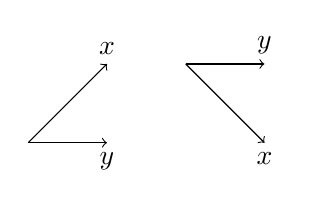
\begin{tikzpicture}
        \draw[->] (-1, 0) -- (0, 1) node[anchor=south] {$x$};
        \draw[->] (-1, 0) -- (0, 0) node[anchor=north] {$y$};

        \draw[->] (1, 1) -- (2, 1) node[anchor=south] {$y$};
        \draw[->] (1, 1) -- (2, 0) node[anchor=north] {$x$};
    \end{tikzpicture}

    \captionof{figure}{Two pair of vectors $B_1$ and $B_2$}
    \label{fig:orientation_of_vectors}
\end{center}

$B_1$ and $B_2$ are both bases of $\R^2$, but if we try to \say{continuously} transform one into the other by \say{rotating} the vectors
while keeping them a basis we will see that at some point we will have $\munderbar{x} \cdot \munderbar{y} = 0$,
hence the two vectors no longe form a basis.

We call this propriety the \textbf{orientation} of the basis.
When we choose the orientation of the axis of a space we are choosing the orientation of the basis.

By convention we say that the positive orientation of the basis is the one defined by the right-hand rule.

We can extend this concept to $\R^d$ by considering the determinant of the matrix of the vectors.

\subsection{Determinant}

Determinants have been covered already in linear algebra, for definition and proprieties see those notes.
We will discuss here some of their geometric proprieties that weren't covered before.

In $\R^2$ the determinant of a matrix of two vectors is the area of the parallelogram defined by the two vectors.
In $\R^3$ it is the volume of the parallelepiped defined by the three vectors.

\begin{gather*}
    \det \left( \begin{pmatrix}
            \munderbar{x} & \munderbar{y}
        \end{pmatrix} \right) = \text{ area} \\
    \det \left( \begin{pmatrix}
            \munderbar{x} & \munderbar{y} & \munderbar{z}
        \end{pmatrix} \right) = \text{ volume}
\end{gather*}

\subsubsection{Cross product}

\textbf{\underline{Definition} (cross product)}: Let $\munderbar{x} = \begin{pmatrix}
        x_1 \\ x_2 \\ x_3
    \end{pmatrix}$ and $\munderbar{y} = \begin{pmatrix}
        y_1 \\ y_2 \\ y_3
    \end{pmatrix}$.
The cross product of $\munderbar{x}$ and $\munderbar{y}$ is the vector

$$
    \munderbar{x} \times \munderbar{y} = \begin{pmatrix}
        x_2 y_3 - x_3 y_2 \\
        x_3 y_1 - x_1 y_3 \\
        x_1 y_2 - x_2 y_1
    \end{pmatrix}
$$

\subsubsection{Cross product and determinant}

\textbf{\underline{Theorem}}: Let $\munderbar{x}, \munderbar{y}, \munderbar{z} \in \R^3$. Then

$$
    \det \left( \begin{pmatrix}
            \munderbar{x} & \munderbar{y} & \munderbar{z}
        \end{pmatrix} \right) = (\munderbar{x} \times \munderbar{y}) \cdot \munderbar{z}
$$

\begin{proof}
    We have that

    \begin{align*}
        \det \left( \begin{pmatrix}
                            \munderbar{x} & \munderbar{y} & \munderbar{z}
                        \end{pmatrix} \right)
         & = \det \begin{pmatrix}
                      x_1 & y_1 & z_1 \\
                      x_2 & y_2 & z_2 \\
                      x_3 & y_3 & z_3
                  \end{pmatrix}                                                        \\
         & = z_1 \det \begin{pmatrix}
                          x_2 & y_2 \\
                          x_3 & y_3
                      \end{pmatrix}
        - z_2 \det \begin{pmatrix}
                       x_1 & y_1 \\
                       x_3 & y_3
                   \end{pmatrix}
        + z_3 \det \begin{pmatrix}
                       x_1 & y_1 \\
                       x_2 & y_2
                   \end{pmatrix}                                                        \\
         & = z_1 (x_2 y_3 - x_3 y_2) - z_2 (x_1 y_3 - x_3 y_1) + z_3 (x_1 y_2 - x_2 y_1) \\
         & = \begin{pmatrix}
                 z_1 \\ z_2 \\ z_3
             \end{pmatrix} \cdot (\munderbar{x} \times \munderbar{y})
    \end{align*}

    The last steps follow from the definition of determinant for $2 \times 2$ matrixes and the definition of the cross product.
\end{proof}

\section{Class of 15/02/2024}

\subsection{Proprieties of the cross product}

\textbf{\underline{Proposition} (characterization of the cross product)}:

\begin{enumerate}
    \item $\munderbar{x} \times \munderbar{y}$ is orthogonal to $\munderbar{x}$ and $\munderbar{y}$.
    \item $\norm{\munderbar{x} \times \munderbar{y}} = \norm{\munderbar{x}} \norm {\munderbar{y}} \abs{\sin \theta}$
          where $\theta$ is the angle between $\munderbar{x}$ and $\munderbar{y}$.
    \item $\det (\munderbar{x}, \munderbar{y}, \munderbar{x} \times \munderbar{y}) \geq 0$
          so that the basis $\munderbar{x}, \munderbar{y}, \munderbar{x} \times \munderbar{y}$ is positively oriented.
\end{enumerate}

\begin{proof}
    We will prove the proprieties one by one.
    These proofs will make heavy use of the definition of the cross product and the determinant from above.
    \begin{enumerate}
        \item From the definition of cross product and knowing that the determinant of a matrix is 0 if two rows are equal we have
              \begin{itemize}
                  \item $(\munderbar{x} \times \munderbar{y}) \cdot \munderbar{x} = \det (\munderbar{x}, \munderbar{y}, \munderbar{x}) = 0$
                  \item $(\munderbar{x} \times \munderbar{y}) \cdot \munderbar{y} = \det (\munderbar{x}, \munderbar{y}, \munderbar{y}) = 0$
              \end{itemize}
        \item Let $\munderbar{z}$ be a vector normal to $\munderbar{x}$ and $\munderbar{y}$, with $\norm{\munderbar{z}} \ne 0$.
              We have that $\abs{\det (\munderbar{x}, \munderbar{y}, \munderbar{z})} = \abs{(\munderbar{x} \times \munderbar{y}) \cdot \munderbar{z}}$.
              Recall that the formula to compute the area of a parallelogram is $\norm{\munderbar{x}} \norm{\munderbar{y}} \abs{\sin \theta}$.
              Since $\det (\munderbar{x}, \munderbar{y}, \munderbar{z})$ is the volume of the parallelepiped defined by the three vectors we have that
              $\abs{\det (\munderbar{x}, \munderbar{y}, \munderbar{z})} = \left(\norm{\munderbar{x}} \norm{\munderbar{y}} \abs{\sin \theta}\right) \cdot \norm{\munderbar{z}}$ just by using the normal formula for the volume (area of base times height).
              Because of (1) we have that $\sin \theta = 1$ and simplifying $\norm{\munderbar{z}}$ we get the result.
        \item We have that $\det (\munderbar{x}, \munderbar{y}, \munderbar{x} \times \munderbar{y}) = \norm{\munderbar{x} \times \munderbar{y}}^2 \geq 0$.
    \end{enumerate}
\end{proof}

\textbf{\underline{Proposition} (proprieties of the cross product)}:
Let $\munderbar{x}, \munderbar{y}, \munderbar{z} \in \R^3$ and $a, b \in \R$. Then

\begin{enumerate}
    \item \textit{Bilinearity}: $(a \munderbar{x} + b \munderbar{y}) \times \munderbar{z} = a (\munderbar{x} \times \munderbar{z}) + b (\munderbar{y} \times \munderbar{z})$ and $\munderbar{x} \times (a \munderbar{y} + b \munderbar{z}) = a (\munderbar{x} \times \munderbar{y}) + b (\munderbar{x} \times \munderbar{z})$.
    \item \textit{Asymmetry}: $\munderbar{x} \times \munderbar{y} = - \munderbar{y} \times \munderbar{x}$.
    \item \textit{Linear independence}: $\munderbar{x} \times \munderbar{y} = \munderbar{0} \iff \munderbar{x}$ and $\munderbar{y}$ are linearly dependent.
\end{enumerate}

\begin{proof}
    To prove (1) and (2) we just apply the definition of the cross product and the determinant.

    For (3) we have
    \begin{align*}
        \norm{\munderbar{x} \times \munderbar{y}} = 0
         & \iff
        \norm {\munderbar{x}} \norm{\munderbar{y}} \abs{\sin \theta} = 0                                        \\
         & \iff \abs{\sin \theta} = 0 \text{ or } \norm{\munderbar{x}} = 0 \text{ or } \norm{\munderbar{y}} = 0 \\
         & \iff \munderbar{x} \text{ and } \munderbar{y} \text{ are linearly dependent}
    \end{align*}

\end{proof}

\subsection{Parametrization}

TODO

\section{Class of 16/02/2024}

\subsection{Parametrizing ellipses}

Last class we saw how to parametrize lines and circles, now we will have a look at ellipses.

An ellipse is defined by the parametrization

\[
    \begin{cases}
        x = a \cos t \\
        y = b \sin t
    \end{cases}
\]

where $a$ and $b$ are the semi-axes of the ellipse. Note that if $a = b$ we get a circle of radius $a$.

For the equation we have

$$
    \frac{x^2}{a^2} + \frac{y^2}{b^2} = 1
$$

The ellipse is the image of the unit circle by tge linear transformation $\begin{pmatrix}
        x \\ y
    \end{pmatrix} \to \begin{pmatrix}
        ax \\ by
    \end{pmatrix}$.

\subsubsection{Applying transformations to curves}

Consider curve $\gamma_1$ which we want to rotate by an angle $\theta$ to obtain $\gamma_2$.

Remember the rotation matrix

$$
    R(\theta) = \begin{pmatrix}
        \cos \theta & -\sin \theta \\
        \sin \theta & \cos \theta
    \end{pmatrix}
$$

For the parametrization is quite easy since we just need to multiply the vector by the rotation matrix.

$$
    \begin{pmatrix}
        x \\ y
    \end{pmatrix} = \begin{pmatrix}
        \cos \theta & -\sin \theta \\
        \sin \theta & \cos \theta
    \end{pmatrix} \begin{pmatrix}
        f(t) \\ g(t)
    \end{pmatrix}
$$

Getting the equation is a bit trickier.
We have to invert the transformation matrix:
consider a point $(x, y)$ on $\gamma_2$, we have that $(x, y) = R(\theta) (x', y')$, hence $(x', y') \in \gamma_1 = R(-\theta) (x, y)$.
We have that $(x,y) \in \gamma_2 \iff R(-\theta)(x, y) \in \gamma_1$.
Now we have $(x', y')$ in terms of $(x, y)$ and we can plug the result of the reverse transformation into the equation of $\gamma_1$.

\subsection{Cylinders}

Let $(x, y, z) \in \R^3$. We have that $\sqrt{x^2 + y^2 + z^2}$ is the distance from the origin and $\sqrt{x^2 + y^2}$ is the distance to the $Oz$ axis.

The equation of a cylinder is

$$
    \left\{ (x, y, z) \in \R^3  : x^2 + y^2 = r^2\right\}
$$

we are basically saying that the distance from the $Oz$ axis is constant and is equal to $r$.

\subsection{Cones}

The way we describe cones is by saying that if we slice the cone at altitude $z$ we will have a circle of radius $z$ and center at $(0,0,z)$.

So we want $\sqrt{x^2 + y^2} = |z|$, hence

$$
    \left\{ (x, y, z) \in \R^3 : x^2 + y^2 = z^2 \right\}
$$

\subsubsection{Variations of the cone}

We can consider the following variations

$$
    x^2 + y^2 = z^2 + 1 \\
    x^2 + y^2 = z^2 - 1
$$

In the first one we have that at $z=0$ we have a circle of radius 1, in the second one we have that at $z=0$ we have a circle of radius $-1$ which is not possible, hence the second equation only gets to $z = \pm 1$.

These type of surfaces are called hyperboloids of revolution.

% TODO: Add the drawings

\subsection{Parametric curves}

We can now give a formal definition of a parametric curve.

\underline{Definition}: A parametric curve $\gamma$ is a function of $t \in I \subseteq \R$ and valued in $\R^d$.

$$
    \gamma(t) = \begin{pmatrix}
        \gamma_1(t) \\
        \vdots      \\
        \gamma_d(t)
    \end{pmatrix} \in \R^d
$$

where $\gamma_1, \ldots, \gamma_d$ are the coordinate functions defined as $\gamma_i: I \to \R$.

Parametric curves are basically the description of the motion of a point in space as a function of time.

\underline{Definition}: The \textbf{domain of definition} of $\gamma$ is the intersection of the domains of the coordinate functions.

\subsubsection{How to represent a curve}

There are many ways to represent a curve, for example we could graph the individual coordinate functions but this is not very representative of the curve itself.

We can try to use a graph to represent a curve $\gamma$:

\underline{Definition}: The \textbf{graph} of $\gamma$ is the subset of $\R^{d+1}$ made of points
$$
    (t, \gamma(t)) = (t, \gamma_1(t), \ldots, \gamma_d(t))
$$
for $t \in I$.

The graphs contains all the information about the curve, but it is not very practical to use because of its complexity.

\underline{Definition}: The \textbf{image} of $\gamma$ is the subset of $\R^d$ made of points $\gamma(t)$ for $t \in I$.

The image is basically the graphs seen from the $x$ axis.

This representation is quite practical but we are losing some information about the parameter $t$, this is mostly ok though.

Note that different curves will always have different graphs but might have the same image.

\underline{Remark}: Every graph is the image of some function in $\R^{d+1}$, but not all images are graphs of some function in $\R^{d-1}$.

\section{Class of 19/02/2024}

\subsection{Continuity and differentiability for parametric curves}

\textbf{\underline{Definition} (continuity)}: Let $\gamma: t \to (\gamma_1, \gamma_2, \ldots, \gamma_d) \in R^d$ be a parametric curve.
$\gamma$ is continuous at $t_0 \in I$ if all the functions $\gamma_1, \ldots, \gamma_d$ are continuous at $t_0$.

\textbf{\underline{Definition} (differentiability)}: Let $\gamma: t \to (\gamma_1, \gamma_2, \ldots, \gamma_d) \in R^d$ be a parametric curve.
$\gamma$ is differentiable at $t_0 \in I$ if all the functions $\gamma_1, \ldots, \gamma_d$ are differentiable at $t_0$.
We define $\gamma'(t_0) = (\gamma_1'(t_0), \ldots, \gamma_d'(t_0))$.

\textbf{\underline{Definition} (speed)}: Let $\gamma: t \to (\gamma_1, \gamma_2, \ldots, \gamma_d) \in R^d$ be a parametric curve differentiable at $t_0 \in I$.
Its speed at $t_0$ is $\norm{\gamma'(t_0)}$.

\underline{Example}: consider the unit circle $\gamma(t) = (\cos t, \sin t)$, we have that

$$
    \gamma'(t) = (-\sin t, \cos t)
$$

and
$$
    \norm{\gamma'(t)} = \sqrt{(-\sin t)^2 + \cos^2 t} = 1
$$

\textbf{\underline{Definition} (higher order differentiability)}:
The parametric curve $\gamma$ is $k$ times differentiable at $t_0 \in I$ if all the functions $\gamma_1, \ldots, \gamma_d$ are $k$ times differentiable at $t_0$.

Note that in physics we sometimes use $\dot{o}, \ddot{o}, \ldots$ to denote the derivative of a function with respect to time.

\subsection{Taylor expansion and local behavior}

\textbf{\underline{Definition} (regular point)}:
If $\gamma: I \to \R^d$ is differentiable at $t_0 \in I$, we say that $t_0$ is a regular point if $\gamma'(t_0) \neq \munderbar{0}$.

\textbf{\underline{Definition} (tangent line)}:
If $\gamma$ is differentiable and $t_0$ is a regular point, the tangent to the image of $\gamma$ at $\gamma(t_0)$ is the line passing through $\gamma(t_0)$ and directed by $\gamma'(t_0)$.
That is

$$
    h \in R \mapsto \gamma(t_0) + h \gamma'(t_0) \in \R^d
$$

\subsubsection{Equation of a line}

We can write the equation of a line from a point and a normal vector:

$$
    \left(
    \begin{pmatrix}
            x \\ y
        \end{pmatrix} - \begin{pmatrix}
            x_0 \\ y_0
        \end{pmatrix}
    \right) \cdot \begin{pmatrix}
        a \\ b
    \end{pmatrix} = 0
$$

where $\begin{pmatrix}
        a \\ b
    \end{pmatrix}$ is the normal vector to the line and $\begin{pmatrix}
        x_0 \\ y_0
    \end{pmatrix}$ is a point on the line.


\underline{Example} (unit circle):
Consider the tangent on the unit circle. We have that its parametrization is
$$
    h \mapsto \begin{pmatrix}
        \cos t_0 \\ \sin t_0
    \end{pmatrix} + h \begin{pmatrix}
        -\sin t_0 \\ \cos t_0
    \end{pmatrix} =
    \begin{pmatrix}
        \cos t_0 - h \sin t_0 \\
        \sin t_0 + h \cos t_0
    \end{pmatrix}
$$

In the case of the unit circle the normal vector is

$$
    \begin{pmatrix}
        a \\ b
    \end{pmatrix}
    =
    \begin{pmatrix}
        -\cos t_0 \\ -\sin t_0
    \end{pmatrix}
    =
    - \gamma(t_0)
$$

(Note that this is the case only for the unit circle.)

We have that the equation of the tangent line of the unit circle at $t_0$ is

$$
    \left(
    \begin{pmatrix}
            x \\ y
        \end{pmatrix} - \begin{pmatrix}
            \cos t_0 \\ \sin t_0
        \end{pmatrix}
    \right)
    \cdot
    \begin{pmatrix}
        -\cos t_0 \\ -\sin t_0
    \end{pmatrix}
    = 0
$$

\underline{Example} ($t_0$ is not a regular point):
Let $\gamma(t) = (t^2, t^3)$, which is continuous and differentiable.
Let $t_0 = 0$, we that $\gamma'(t_0) = \munderbar{0}$.
We have that
$$
    \begin{cases}
        y = x^{3/2}  & \text{ if } t \geq 0 \\
        y = -x^{3/2} & \text{ if } t \leq 0
    \end{cases}
$$

with $x \geq 0$. We see how $\gamma'(t_0)$ exists but is not regular.

We call this an \textbf{ordinary cusp} (formal definition later).

\begin{figure}[H]
    \centering
    \subfloat[\centering Image]{{
                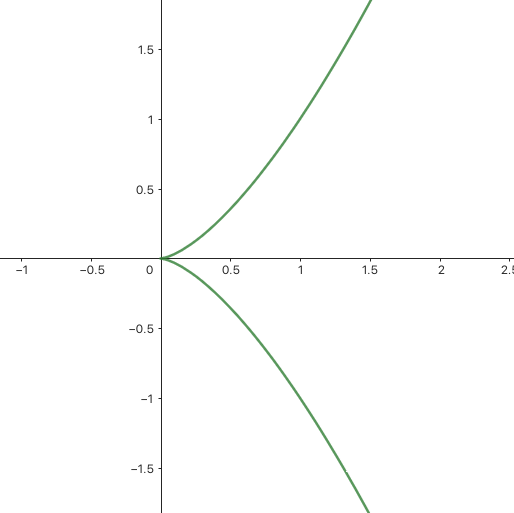
\includegraphics[width=0.35\textwidth]{assets/analysis_2/ordinary_cusp_image.png}
            }}
    \subfloat[\centering Graph]{{
                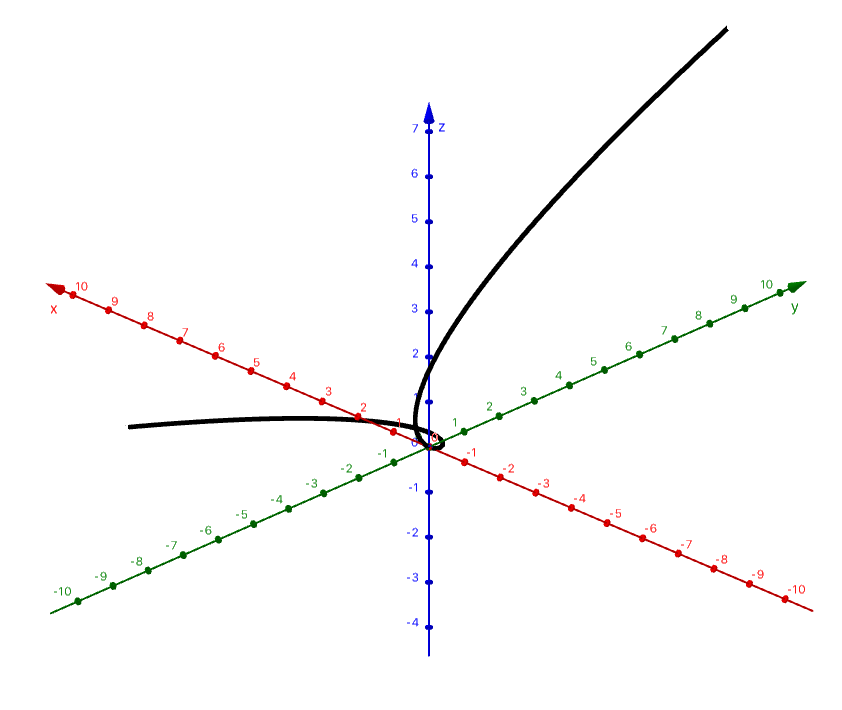
\includegraphics[width=0.35\textwidth]{assets/analysis_2/ordinary_cusp_graph.png}
            }}
    \caption{Ordinary cusp}
    \label{fig:ordinary_cusp}
\end{figure}

\subsubsection{Taylor expansion}

\textbf{\underline{Definition} (Taylor expansion)}:
Let $\gamma: I \to \R^d$ be $k$ times differentiable over $I$.
Then

$$
    \gamma(t_0 + h) =
    \gamma(t_0) +
    h \gamma'(t_0) +
    \frac{h^2}{2!} \gamma''(t_0) +
    \ldots +
    \frac{h^k}{k!} \gamma^{(k)}(t_0) +
    o(h^k)
$$

From this definition we see that the image of $\gamma$ is close to $\gamma (t_0)$ since it is the principal term of the expansion.

Moreover note that the Taylor expansion of order 1 with $\gamma'(t_0) \ne \munderbar{0}$ is

$$
    \gamma(t_0 + h) = \gamma(t_0) + h \gamma'(t_0) + o(h)
$$

which is the equation of the tangent line.

\subsubsection{Local behavior}

We can use the Taylor expansion to study the behavior of a curve in the neighborhood of $t_0$.

% TODO: add graphs

\textbf{\underline{Definition} (biregular point)}:
Let $\gamma: I \to \R^d$ such that $\gamma'(t_0) \ne \munderbar{0}$ and $\gamma''(t_0)$ is linearly independent from $\gamma'(t_0)$.
Then we say that $t_0$ is a biregular point.

\textbf{\underline{Definition} (inflection point)}:
$t_0$ is an inflection point if $\gamma'(t_0) \ne \munderbar{0}$ but $\gamma''(t_0)$ is linearly dependent from $\gamma'(t_0)$.

This means that the curve crosses the tangent line at $t_0$.


\textbf{\underline{Definition} (ordinary cusp)}:
$t_0$ is an ordinary cusp if $\gamma'(t_0) = \munderbar{0}$ but $\gamma''(t_0), \gamma'''(t_0)$ are linearly independent.

\begin{figure}[H]
    \centering
    \subfloat[\centering Inflection point]{{
                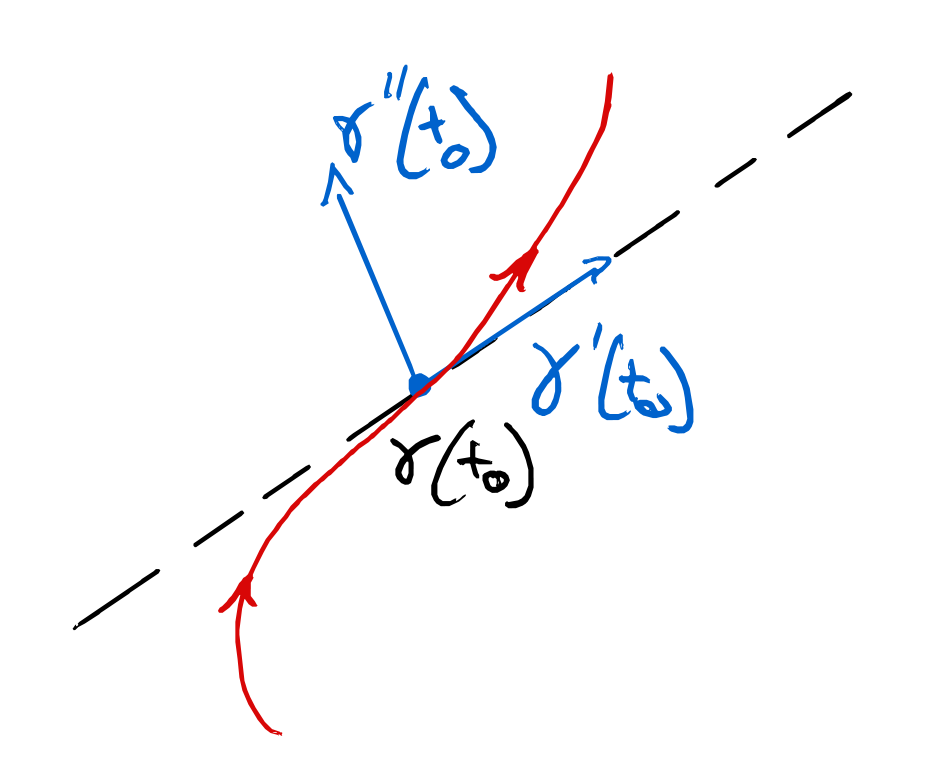
\includegraphics[width=0.35\textwidth]{assets/analysis_2/inflection_point.png}
            }}
    \subfloat[\centering Ordinary cusp]{{
                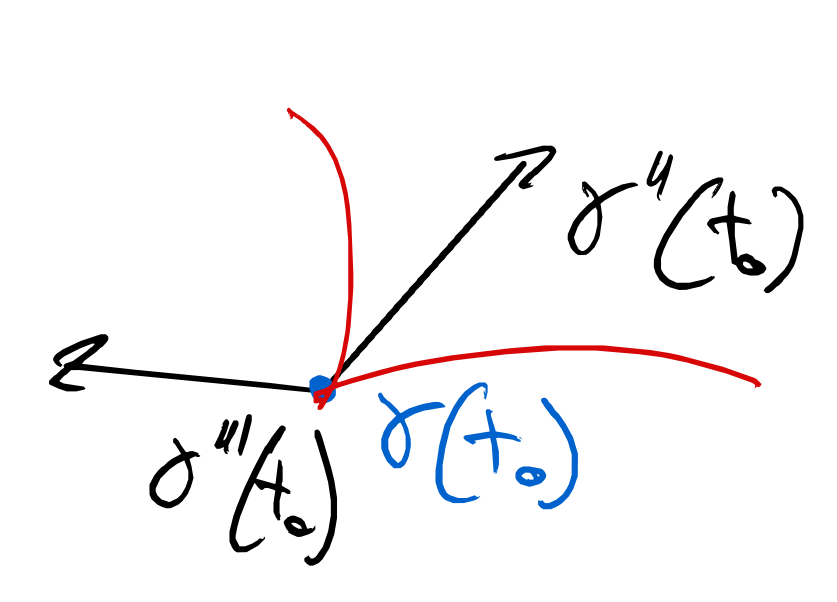
\includegraphics[width=0.35\textwidth]{assets/analysis_2/ordinary_cusp.png}
            }}
    \caption{Inflection point and ordinary cusp}
    \label{fig:inflection_point_and_ordinary_cusp}
\end{figure}

\section{Class of 21/02/2024}

\textbf{\underline{Lemma} ($\gamma'$ and $\gamma''$)}:
If $\gamma: I \to \R^d$ is of class $C^2$ then

$$
    \gamma'(t) \cdot \gamma''(t) = \dv{t}\left(\frac{1}{2}\norm{\gamma'(t)}^2\right)
$$

A direct consequence of this is that $\forall t \in I$, $\gamma'(t) \cdot \gamma''(t) = 0 \iff t \mapsto \norm{\gamma'(t)}^2$ is constant.

\begin{proof}
    We have that

    \begin{align*}
        \dv{t}\norm{\gamma'(t)}^2 & = \dv{t}(\gamma'(t) \cdot \gamma'(t))                         \\
                                  & = \gamma''(t) \cdot \gamma'(t) + \gamma'(t) \cdot \gamma''(t) \\
                                  & = 2 \gamma''(t) \cdot \gamma'(t)
    \end{align*}
\end{proof}

\subsection{Mean value theorem}

Recall the mean value theorem for functions of one variable:

\begin{itemize}
    \item If $f : [a, b] \to \R$ is differentiable then $\exists c \in (a, b)$ such that

          $$
              f'(c) = \frac{f(b) - f(a)}{b - a}
          $$

    \item If $f$ is of class $C^1$ then $\exists c \in (a, b)$ such that

          $$
              f(b) - f(a) = \int_a^b f'(x) \dd{x}
          $$
\end{itemize}

Note that for curves the first point is \textbf{not} generally true.
Consider as counterexample $\gamma(t) = \begin{pmatrix}
        \cos t \\ \sin t
    \end{pmatrix}$ with $t \in [0, 2\pi]$.
We have in fact that $ \frac{\gamma(2\pi) - \gamma(0)}{2\pi - 0} = \munderbar{0}$ which is not equal to $\gamma'(t)$ for any $t$.

However the second point is still true.

\textbf{\underline{Theorem} (mean value theorem)}:
If $\gamma$ is of class $C^1$ then

$$
    \gamma(b) - \gamma(a) = \int_a^b \gamma'(t) \dd{t}
$$

where $\int_a^b \gamma'(t) \dd{t}$ is the vector in $\R^d$ whose $i$-th component is $\int_a^b \gamma_i'(t) \dd{t}$.

\subsection{Curves in polar coordinates}

\textbf{\underline{Definition} (polar coordinates functions)}:
Let $I \subseteq \R$ and $g: I \to [0, +\infty)$ be a non-negative function.
The curve $r = g(\theta)$ is the real valued function

$$
    \gamma: \theta \in I \to g(\theta) \begin{pmatrix}
        \cos \theta \\ \sin \theta
    \end{pmatrix} \in \R^2
$$

Let's now introduce

$$
    e_r = \begin{pmatrix}
        \cos \theta \\ \sin \theta
    \end{pmatrix},
    \quad
    e_\theta = \begin{pmatrix}
        -\sin \theta \\ \cos \theta
    \end{pmatrix}
$$

These two vectors represent the basis of the polar coordinates system.

\textbf{\underline{Lemma} ($e_r$ and $e_\theta$)}:
\begin{itemize}
    \item $\forall \theta \in I$, $e_r \cdot e_\theta = 0$.
    \item $\theta \mapsto e_r(\theta)$ and $\theta \mapsto e_\theta(\theta)$ are class $C^\infty$ and $e_r' = e_\theta$, $e_\theta' = -e_r$.
\end{itemize}

\begin{proof}
    We use the lemma discussed at the beginning of the class:

    TODO
\end{proof}

\textbf{\underline{Lemma}}: Let $g: I \subseteq \R \to [0, +\infty)$ of class $C^2$.
Then the curve $\gamma: \theta \mapsto g(\theta) e_r(\theta)$ is of class $C^2$ and

\begin{align*}
    \gamma'  & = g' e_r + g e_\theta                         \\
    \gamma'' & = g'' e_r + g' e_\theta + g' e_\theta - g e_r \\
             & = (g'' - g) e_r + 2 g' e_\theta
\end{align*}


\textbf{\underline{Remark}}:
\begin{align*}
    \text{a point $\theta_0$ is regular} & \iff \gamma'(\theta_0) \ne \munderbar{0}                                           \\
                                         & \iff g'(\theta_0) e_r(\theta_0) + g(\theta_0) e_\theta(\theta_0) \ne \munderbar{0} \\
                                         & \iff \begin{pmatrix}
                                                    g'(\theta_0) \\ g(\theta_0)
                                                \end{pmatrix} \ne \begin{pmatrix}
                                                                      0 \\ 0
                                                                  \end{pmatrix}                                              \\
                                         & \iff g'(\theta_0) \ne 0
\end{align*}

\begin{proof}
    TODO, just show the calculations, it's just a bunch of derivatives.
\end{proof}

\begin{proof}
    The first steps are just the definition of regular point and deriving $\gamma$.

    The last step is true because we know that $g \geq 0$ by definition, hence if $g = 0$ then it is a minimum and $g' = 0$.
\end{proof}

\subsection{Bezier curves and splines}

Bezier curves are a way for computers to represent curves.
We use a set of control points we can move around to change the shape of the curve.

By convention $t$ is in $[0, 1]$. We will look at the cases for 2 and 3 control points and then generalize to $n$ control points.

\begin{description}
    \item[2 points] We have $P_0$ and $P_1$.
        In this case there isn't much to do, we just have a line from $P_0$ to $P_1$. The parametrization is

        $$
            \gamma(t) = (1 - t) \munderbar{P_0} + t \munderbar{P_1}
        $$

    \item[3 points] We have $P_0$, $P_1$ and $P_2$.
        We could just draw straight lines from $P_0$ to $P_1$ and from $P_1$ to $P_2$ but we want to have a smooth curve.

        Let $\gamma_{0,1}$ and $\gamma_{1,2}$ be the parametrizations of the lines from $P_0$ to $P_1$ and from $P_1$ to $P_2$.
        Then $\gamma_{0,1,2}$ will be the interpolation between $\gamma_{0,1}$ and $\gamma_{12}$.

        \begin{align*}
            \gamma_{0,1,2}(t) & = (1 - t) \gamma_{0,1}(t) + t \gamma_{1,2}(t)                                                                                   \\
                              & = (1 - t) \left((1 - t) \munderbar{P_0} + t \munderbar{P_1}\right) + t \left((1 - t) \munderbar{P_1} + t \munderbar{P_2}\right)
        \end{align*}

    \item[General case] We define this by recursion:
        \begin{itemize}
            \item $\gamma_{0,1}(t) = (1 - t) \munderbar{P_0} + t \munderbar{P_1}$
            \item $\gamma_{0,1, \ldots, n}(t) = (1 - t) \gamma_{0,1, \ldots, n}(t) + t \gamma_{1,2, \ldots, n+1}(t)$
        \end{itemize}
\end{description}

\textbf{\underline{Lemma}}:
For every $t \in [0, 1]$

$$
    \gamma_{0,1, \ldots, n}(t) = \sum_{k=0}^n \binom{n}{k} (1 - t)^{n-k} t^k \munderbar{P_k}
$$

We see how this is a polynomial of class $C^\infty$. It is also very easy to compute the derivative and the bounding box of the curve.

You can find many animations of Bezier curves on the internet, such as this one: \url{https://www.jasondavies.com/animated-bezier/}.

\subsubsection{Spines}

Spines are a generalization of Bezier curves.

\textbf{\underline{Definition}}: Let $\Psi_{k, n}: [0, 1]\to [0, 1]$ such that

$$
    \gamma_{0,1, \ldots, n}(t) = \sum_{k=0}^n \Psi_{k, n}(t) \munderbar{P_k}
$$

with $\sum_{k=0}^n \Psi_{k, n}(t) = 1$.

See \url{https://www.ibiblio.org/e-notes/Splines/basis.html} for animations of spines.

\section{Class of 22/02/2024 - Notions of topology}


\subsection{Introduction to path integrals}

This is not part of this section of the course but we are doing it now because we will use it in physics very soon.

Let $\gamma: t \in I \to \R^d$ with $d = 1, 2, 3$.
If $\gamma(t)$ is the position at time $t$, then $\gamma'(t) = \dot{\gamma}(t)$ is the velocity, $\gamma''(t) = \ddot{\gamma}(t)$ is the acceleration and the image of $\gamma$ is the trajectory.

Many times in physics we have differential equations of the form

$$
    m \ddot{\gamma} = F(\gamma, \dot{\gamma}, t)
$$

We might use path integrals of a vector fields, for example, to calculate the work done by a force along a trajectory.

Consider the force vector field:

\begin{align*}
    \munderbar{F}: \R^d & \to \R^d                \\
    F(x,y)              & = \begin{pmatrix}
                                F_1(x, y) \\ F_2(x, y)
                            \end{pmatrix}
\end{align*}

\textbf{\underline{Definition} (path integral)}:

$$
    \int_\gamma \munderbar{F} \cdot \dd{\munderbar{s}} = \int_a^b \munderbar{F}(\gamma(t)) \cdot \gamma'(t) \dd{t}
$$

From this formula we obtain 2 results that we will not prove yet because we don't have the tools but they are important to know:

\begin{itemize}
    \item The result does not depend on the speed of the curve, only on the trajectory.
    \item If $\munderbar{F} = \nabla g$ (with $g: \R^2 \to \R$) is the gradient of a potential $g$, then $\int_\gamma \munderbar{F} \cdot \dd{\munderbar{s}} = \int_\gamma \nabla g \cdot \dd{\munderbar{s}} = g(\gamma(b)) - g(\gamma(a))$.

          If $g = g(x, y)$ then we have that $\nabla g = \begin{pmatrix}
                  \pdv{g(x, y)}{x} \\ \pdv{g(x,y)}{y}
              \end{pmatrix}$.

          Note that this is basically the extension of the fundamental theorem of calculus in higher dimensions.
\end{itemize}

\subsection{Topology in higher dimensions}

\subsubsection{Useful notions}

We recall some notions we saw earlier in the course:

\begin{itemize}
    \item $\norm{\munderbar{x}} \in [0,+\infty)$ with $\munderbar{x} \in \R^d$ (norm).
    \item $\norm{\munderbar{x} + \munderbar{y}} \leq \norm{\munderbar{x}} + \norm{\munderbar{y}}$ (triangle inequality).
    \item $\norm{a \munderbar{x}}$ = $\abs{a} \norm{\munderbar{x}}$.
    \item $\norm{\munderbar{x}} = 0 \iff \munderbar{x} = \munderbar{0}$.
\end{itemize}

\textbf{\underline{Definition} (distance)}: If $\munderbar{x}, \munderbar{y} \in \R^d$ then the distance between $\munderbar{x}$ and $\munderbar{y}$ is

$$
    d = \norm{\munderbar{x} - \munderbar{y}} \in \R
$$

\subsubsection{Limits}

\textbf{\underline{Definition} (limits in $\R^d$)}:
We say that a sequence in $\R^d$, $\left(\munderbar{x}_n\right)_{n \in \N}$ converges to $\munderbar{a} \in \R^d$ if the real-valued sequence $\left(\norm{\munderbar{x}_n - \munderbar{a}}\right)_{n \in \N}$ converges to 0.

We can also define limits using the usual $\varepsilon - N$ characterization: $\left(\munderbar{x}_n\right)_{n \in \N}$ converges to $\munderbar{a} \in \R^d$ iff

$$
    \forall \varepsilon > 0, \exists N \in \N : n \geq N \implies \norm{\munderbar{x}_n - \munderbar{a}} < \varepsilon
$$

Geometrically, this means considering a ball of radius $\varepsilon$ centered at $\munderbar{a}$, then all the points of the sequence will eventually be inside the ball.

\textbf{\underline{Proposition}}:
Let $\munderbar{x}_n = \begin{pmatrix}
        x_{n,1} \\ \vdots \\ x_{n,d}
    \end{pmatrix}$.

$\left(\munderbar{x}_n\right)_{n \in \N}$ converges iff for $i \in \{1, \ldots, d\}$, $\left(x_{n,i}\right)_{n \in \N}$ converges to $a_i$ as $n \to +\infty$.

\begin{proof}
    \skiplineafterproof
    \begin{description}
        \item[$\implies$]
            Assume $\norm{\munderbar{x}_n - \munderbar{a}}$ converges to 0.
            Fix $i \in \{1, \ldots, d\}$.
            Note that

            $$
                \sum_{j = 1}^d \left(x_{j, n} - a_j\right)^2 \geq \left(x_{i, n} - a_i\right)^2
            $$

            So if we take the square root we get that

            $$
                \norm{\munderbar{x}_n - \munderbar{a}} \geq \abs{x_{i, n} - a_i}
            $$

            So since $\norm{\munderbar{x}_n - \munderbar{a}}$ converges to 0 we have that $\abs{x_{i, n} - a_i}$ converges to 0 as well, thus $x_{i, n}$ converges to $a_i$.
        \item[$\impliedby$]
            Assume that $\left(x_{n, i}\right)_{n \in \N}$ converges to $a_i$ for $i \in \{1, \ldots, d\}$.
            Let $u_{i, n} = x_{i, n} - a_i$, then $u_{i, n}$ converges to 0.

            We want to prove that

            $$
                \norm{\munderbar{x}_n - \munderbar{a}} = \sqrt{\sum_{i=1}^d \left(x_{i, n} - a_i\right)^2} = \sqrt{\sum_{i=1}^d \left(u_{i, n}\right)^2}
            $$
            converges to 0.

            Since $u_{i, n} \to 0$ then also $\left(u_{i, n}\right)^2 \to 0$.
            Then since the square root is continuous we can apply the transference principle to obtain the result.
    \end{description}
\end{proof}

\textbf{\underline{Definition} (operations on limits)}:
Let $\left(\munderbar{x}_n\right)_{n \in \N}$ and $\left(\munderbar{y}_n\right)_{n \in \N}$ be sequences in $\R^d$ converging to $\munderbar{a}$ and $\munderbar{b}$ respectively.
Then

\begin{enumerate}

    \item $\left(\munderbar{x}_n + \munderbar{y}_n\right)_{n \in \N}$ converges to $\munderbar{a} + \munderbar{b}$.
    \item $\left(\munderbar{x}_n \cdot \munderbar{y}_n\right)_{n \in \N}$ converges to $\munderbar{a} \cdot \munderbar{b}$.
    \item If $d = 3$ then $\left(\munderbar{x}_n \times \munderbar{y}_n\right)_{n \in \N}$ converges to $\munderbar{a} \times \munderbar{b}$.
    \item $\norm{\munderbar{x}_n}$ converges to $\norm{\munderbar{a}}$.
\end{enumerate}

\begin{proof}
    The proof of this is very easy and can be obtained by applying the previous proposition and properties of limits in $\R$.
\end{proof}

\section{Class of 23/02/2024 - Interior and closure}

\subsection{Interior}

\textbf{\underline{Definition} (ball)}:
Let $\munderbar{a} \in \R^d$ and $r \geq 0$.
\begin{itemize}
    \item The open ball of radius $r$ centered at $\munderbar{a}$ is
          $$
              B_o(\munderbar{a}, r) = \left\{ \munderbar{x} \in \R^d : \norm{\munderbar{x} - \munderbar{a}} < r \right\}
          $$
    \item The closed ball of radius $r$ centered at $\munderbar{a}$ is
          $$
              B_c(\munderbar{a}, r) = \left\{ \munderbar{x} \in \R^d : \norm{\munderbar{x} - \munderbar{a}} \leq r \right\}
          $$
\end{itemize}

\textbf{\underline{Definition} (interior)}:
If $V \subseteq \R^d$, we call interior of $V$, written $\mathring{V}$, the set of $n \in \R^d$ such that

$$
    \exists \varepsilon > 0, \enspace
    \forall \munderbar{y} \in B_c(\munderbar{x}, \varepsilon), \enspace
    \munderbar{y} \in V
$$

then

$$
    \munderbar{x} \in \mathring{V} \iff \exists \varepsilon > 0, \enspace
    B_o(\munderbar{x}, \varepsilon) \subseteq V
$$

\subsubsection{Theorem: interior means removing the boundary}

\underline{Statement}: Let $V \subseteq \R^d = \{ (x, y) \in \R^2 : x^2 + y^2 \leq 1 \}$.
Then $\mathring{V} = \{ (x, y) \in \R^2 : x^2 + y^2 < 1 \}$.

\begin{proof}
    We have 3 cases to consider:
    \begin{enumerate}
        \item $x + y < 1$
        \item $x + y = 1$
        \item $x + y > 1$
    \end{enumerate}

    Then
    \begin{enumerate}
        \item $(x, y) \notin V$ so $(x, y) \notin \mathring{V}$. See next proposition for the proof.
        \item Let $(x, y)$ s.t $x + y = 1$.
              For $\varepsilon > 0$ consider $(x, y - \varepsilon)$.
              Then $x + (y - \varepsilon) = 1 - \varepsilon < 1$, thus $(x, y - \varepsilon) \notin V$.
              But $\norm{\begin{pmatrix}
                          x \\ y
                      \end{pmatrix} - \begin{pmatrix}
                          x \\ y - \varepsilon
                      \end{pmatrix}} = \varepsilon$ so $(x, y - \varepsilon) \in B_c((x, y), \varepsilon)$.
              Therefore $(x, y) \notin \mathring{V}$.

        \item Let $(x_0, y_0)$ s.t. $x_0 + y_0 > 1$.
              We know that the direction towards the boundary is $\begin{pmatrix}
                      -1 \\ -1
                  \end{pmatrix}$,
              so the curve $\gamma: t \mapsto \begin{pmatrix}
                      x_0 \\ y_0
                  \end{pmatrix} + t \begin{pmatrix}
                      -1 \\ -1
                  \end{pmatrix}$
              intersects the boundary when $\gamma_1(t) + \gamma_2(t) = 1$.
              That is when $x_0 - t + y_0 - t = 1$ and $t^* = \frac{x_0 + y_0 - 1}{2}$.
              The distance is then $\norm{\gamma(t^*) - \begin{pmatrix}
                          x_0 \\ y_0
                      \end{pmatrix}} = \frac{\sqrt{2}}{2} (x_0 + y_0 - 1)$.
              Therefore for $\varepsilon > 0$ with $\varepsilon < \frac{\sqrt{2}}{2} (x_0 + y_0 - 1)$ we have that $B_o((x_0, y_0), \varepsilon) \subseteq V$, thus $(x_0, y_0) \in \mathring{V}$.
    \end{enumerate}
\end{proof}

\subsubsection{Neighborhoods}

\textbf{\underline{Definition} (neighborhood)}:
If $\munderbar{n} \in \R^d$, a set $V$ is said the neighborhood of $\munderbar{n}$ iff $\munderbar{n} \in \mathring{V}$.

The idea is that when we speak about the interior we fix the set and look at the points inside, while when we speak about neighborhoods we fix the point and look at the sets around it.

\subsubsection{Theorem: relationships between interior and other sets}

\underline{Statement}: Let $V, W \subseteq \R^d$.
Then

\begin{enumerate}
    \item $\mathring{V} \subseteq V$
    \item If $V \subseteq W$ then $\mathring{V} \subseteq \mathring{W}$
\end{enumerate}

\begin{proof}
    \skiplineafterproof
    \begin{enumerate}
        \item Let $\munderbar{x} \in \mathring{V}$.
              Since $\munderbar{x} \in \mathring{V}$ then $\exists \varepsilon > 0$ such that $B_c(\munderbar{x}, \varepsilon) \subseteq V$.
              Thus, since $\munderbar{x} \in B_c(\munderbar{x}, \varepsilon)$ we have that $\munderbar{x} \in V$.
        \item Let $V, W$ such that $V \subseteq W$ let and $\munderbar{x} \in \mathring{V}$.
              Then, by definition, $\exists \varepsilon > 0$ such that $B_c(\munderbar{x}, \varepsilon) \subseteq V$.
              As $V \subseteq W$ then $B_c(\munderbar{x}, \varepsilon) \subseteq V \subseteq W$.
              Therefore $\exists \varepsilon > 0$ such that $B_c(\munderbar{x}, \varepsilon) \subseteq W$.
              Thus $\munderbar{x} \in \mathring{W}$.
    \end{enumerate}
\end{proof}

\subsection{Closure}

\textbf{\underline{Definition} (closure)}:
Let $V \subseteq \R^d$. The closure of $V$, written $\overline{V}$, is the set of $\munderbar{x} \in \R^d$ such that there exists a sequence $\left(\munderbar{x}_n\right)_{n \in \N}$ of elements of $V$ converging to $\munderbar{x}$.

For example on $\R$ the closure of $(0, +\infty)$ is $[0, +\infty)$.

\subsubsection{Theorem: closure adds the boundary}

\underline{Statement}: Let $\munderbar{a} \in \R^d$ and $r > 0$.
Then the closure of $B_o(\munderbar{a}, r)$ is $B_c(\munderbar{a}, r)$.

\begin{proof}
    We have 3 cases

    \begin{enumerate}
        \item $\norm{\munderbar{x} - \munderbar{a}} < r$
        \item $\norm{\munderbar{x} - \munderbar{a}} = r$
        \item $\norm{\munderbar{x} - \munderbar{a}} > r$
    \end{enumerate}

    Then

    \begin{enumerate}
        \item Since $\munderbar{x} \in V$ then $\munderbar{x} \in \overline{V}$. See next proposition for the proof.
        \item Let $\munderbar{x}$ s.t. $\norm{\munderbar{x} - \munderbar{a}} = r$.
              Let $\munderbar{x}_n = \munderbar{x} + t_n(\munderbar{a} - \munderbar{x})$, where we want that $\munderbar{x}_n \to \munderbar{x}$ and $\munderbar{x}_n \in V \enspace \forall n$.
              The first condition is equivalent to saying that $\norm{\munderbar{x}_n - \munderbar{x}} = \norm{t_n(\munderbar{a} - \munderbar{x})} = t_n \norm{\munderbar{a} - \munderbar{x}} \to 0$, therefore we want $t_n \to 0$.
              For the second condition we want that $\norm{\munderbar{x}_n - \munderbar{a}} < r$, which is
              $\norm{\munderbar{x}_n - \munderbar{a}} = \norm{\munderbar{x} + t_n(\munderbar{a} - \munderbar{x}) - \munderbar{a}} = \norm{(\munderbar{x} - \munderbar{a})(1 - t_n)} = r \abs{1 - t_n} < r$. Then this is $< r$ if $t_n \in [0, 1]$.
              We can take $t_n = \frac{1}{2^n}$.
        \item We will prove this one by contradiction. Let $\munderbar{x}$ s.t. $\norm{\munderbar{x} - \munderbar{a}} > r$.
              Take a sequence $\left(\munderbar{x}_n\right)_{n \in \N} \in V$ converging to $\munderbar{x}$.
              This means that $\norm{\munderbar{x}_n - \munderbar{a}} < r$ for any $n$.
              As $\munderbar{x}_n \to \munderbar{x}$ we have that $(\munderbar{x}_n - \munderbar{a}) \to (\munderbar{x} - \munderbar{a})$.
              Then $\norm{\munderbar{x}_n - \munderbar{a}} \to \norm{\munderbar{x} - \munderbar{a}}$.
              So $\lim_{n \to +\infty} \norm{\munderbar{x}_n - \munderbar{a}} = \norm{\munderbar{x} - \munderbar{a}}$, thus $\norm{\munderbar{x} - \munderbar{a}} \leq r$ and we have a contradiction.
    \end{enumerate}
\end{proof}

\subsubsection{Theorem: relationships between closures and other sets}

\underline{Statement}: Let $V, W \subseteq \R^d$.
Then

\begin{enumerate}
    \item $V \subseteq \overline{V}$
    \item If $V \subseteq W$ then $\overline{V} \subseteq \overline{W}$
\end{enumerate}

\begin{proof}
    \skiplineafterproof
    \begin{enumerate}
        \item Let $\munderbar{x} \in V$.
              Then let $\left(\munderbar{x}_n\right)_{n \in \N} = \munderbar{x}$ be a constant sequence of elements of $V$.
              Then $\munderbar{x}_n \to \munderbar{x}$ and $\munderbar{x} \in \overline{V}$.
        \item Let $V, W$ such that $V \subseteq W$ let and $\munderbar{x} \in \overline{V}$.
              Then, by definition, $\exists \left(\munderbar{x}_n\right)_{n \in \N} \in V$ such that $\munderbar{x}_n \to \munderbar{x}$.
              As $V \subseteq W$ then $\munderbar{x}_n \in W$ and $\munderbar{x} \in \overline{W}$.
    \end{enumerate}
\end{proof}

\subsection{Boundary}

\textbf{\underline{Definition} (boundary)}:
If $V \subseteq \R^d$, the (topological) boundary of $V$, written $\partial V$, is the set defined as $\partial V = \overline{V} \setminus \mathring{V}$.

\end{document}